\documentclass[tikz]{standalone}% 'crop' is the default for v1.0, before it was 'preview'
\usepackage{tikz}
\usepackage{pgfplots}
\usepackage{amsmath}

\usepgfplotslibrary{colormaps}
\pgfplotsset{compat=1.18}
\usetikzlibrary{plotmarks}
%\usetikzlibrary{...}% tikz package already loaded by 'tikz' option
\begin{document}


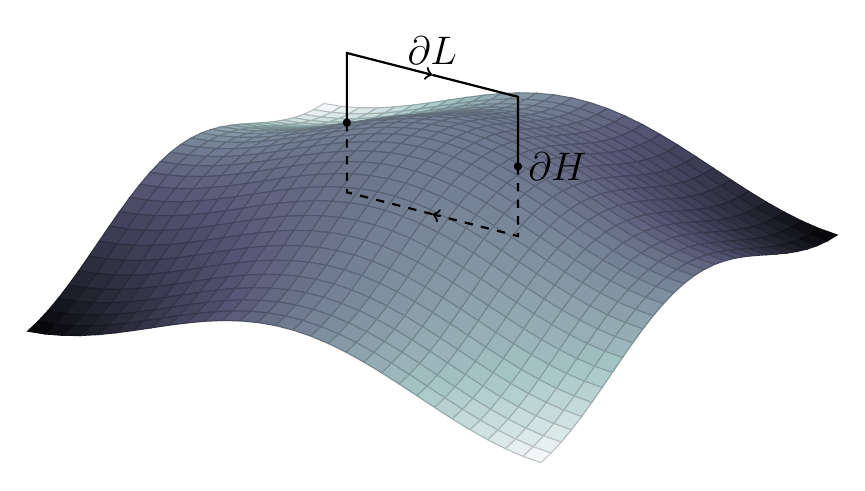
\begin{tikzpicture}[font=\Large]
\begin{axis}[
    hide axis,
    scale=2,
    view={120}{40},
    xmin=-4,xmax=4,
    ymin=-4,ymax=4,
    zmin=-2,zmax=10,
    trig format plots=rad,
  ]
    % Draw big surface
    \addplot3 [ surf, colormap/bone, domain=-3:3, domain y=-3:3, samples=30, samples y=30, variable=\u, variable y=\v, point meta=u*v]
    ( {u}, {v}, {cos(u) + cos(v)} );

    \draw[->, thick, black] (axis cs: 0,-1,{cos(0) + cos(-1)}) -- (axis cs: 0,-1,{cos(0) + cos(-1) + 2}) -- (axis cs: 0,0,{cos(0) + cos(-1) + 2}) node[above] {$\partial L$}; 
    \draw[thick, black] (axis cs: 0,0,{cos(0) + cos(-1) + 2}) -- (axis cs: 0,1,{cos(0) + cos(-1) + 2}) -- (axis cs: 0,1,{cos(0) + cos(1)}) node[right] {$\partial H$};
    \node[circle,fill=black,inner sep=0pt,minimum size=3pt] at (axis cs: 0,1,{cos(0) + cos(1)}) {}; 
    \draw[->, thick, dashed, black] (axis cs: 0,1,{cos(0) + cos(1)}) -- (axis cs: 0,1,{cos(0) + cos(1) - 2})  -- (axis cs: 0,0,{cos(0) + cos(1) - 2}); 
    \draw[thick, dashed, black] (axis cs: 0,0,{cos(0) + cos(1) - 2}) -- (axis cs: 0,-1,{cos(0) + cos(1) - 2})  -- (axis cs: 0,-1,{cos(0) + cos(-1)}); 
    \node[circle,fill=black,inner sep=0pt,minimum size=3pt] at (axis cs: 0,-1,{cos(0) + cos(-1)}) {}; 

\end{axis}

\end{tikzpicture}
\end{document}